\documentclass[journal,10pt,twocolumn]{article}
\usepackage{graphicx}
\usepackage[margin=0.5in]{geometry}
\usepackage{amsmath}
\usepackage{array}
\usepackage{booktabs}
\usepackage{listings}
\providecommand{\norm}[1]{\left\lVert#1\right\rVert}
\providecommand{\abs}[1]{\left\vert#1\right\vert}
\usepackage{enumerate}
\let\vec\mathbf
\newcommand{\myvec}[1]{\ensuremath{\begin{pmatrix}#1\end{pmatrix}}}
\newcommand{\mydet}[1]{\ensuremath{\begin{vmatrix}#1\end{vmatrix}}}
\providecommand{\brak}[1]{\ensuremath{\left(#1\right)}}
\lstset{
frame=single,
breaklines=true,
columns=fullflexible
}
\title{\textbf{Matrix Assignment}}
\author{A L U R U A J A Y}
\date{September 2022}
\begin{document}
\maketitle
\paragraph{\textit{Problem Statement} - Find the equation of the tangent line to the curve
\begin{math}
y=x^2-2x+7
\end{math}
}
\begin{enumerate}
    \item\textbf{parallel to the line 2x-y+9=0.}
    \item\textbf{perpendicular to the line 5y-15x=13.}
\end{enumerate}

\section{Solution}
According to the question equation of a parabola is 
\vspace{0.3cm}\\
\begin{math}
y=x^2-2x+7
\end{math}
\vspace{0.3cm}\\
The standard equation of the parabola is given as :
\begin{align}
\vec{x}^{\top}\vec{V}\vec{x}+2\vec{u}^{\top}\vec{x}+f=0
\end{align}
\begin{math}
\vec{V} \and=\begin{pmatrix}
	1 & 0\\
	0 & 0\\
	\end{pmatrix},\hspace{0.33cm}
    \vec{u}\and=\begin{pmatrix}
	-1 \\
	-0.5 \\
	\end{pmatrix},\hspace{0.33cm}
    f\and=7
    \end{math}
\subsection{parallel to the line 2x-y+9=0}
Normal vector of a given line \begin{math}\vec{n}_1\end{math} = \myvec{2 \\ -1}
\begin{flushleft}
\begin{math}\vec{V}\end{math}\ is not invertible,Then given the normal vector \begin{math}\vec{n}\end{math}\, the point of contact to is given by the matrix equation
\vspace{0.3cm}\\
\begin{equation}
    \myvec{(\vec{u}+k_1\vec{n}_1)^T \\ \vec{V}}\vec{q}_1 = \myvec{-f \\ k_1\vec{n}_1- \vec{u}}
\end{equation}
\begin{math}
\myvec{(\myvec{-1 \\ -0.5} + \frac{1}{2}\myvec{2 \\ -1})^T \vspace{0.3cm}\\ \begin{pmatrix}
	1 & 0\\
	0 & 0\\
	\end{pmatrix}} \vec{q}_1 = \myvec{-7 \vspace{0.3cm}\\ \frac{1}{2}\myvec{2 \\ -1} - \myvec{-1 \\ -0.5}}
\end{math}
\vspace{0.3cm}\\
By solving the above equation,we can get the point of contact as
\vspace{0.3cm}\\
\begin{center}
    \begin{math}
  \vec{q}_1\and=\begin{pmatrix}
	2 \\
	7 \\
	\end{pmatrix}
\end{math}
\end{center}
Tangent Equation is
\begin{equation}
      \vec{n}_1^T(\vec{x}-\vec{q}_1) = 0
\end{equation}
By substituting the values of \begin{math}
  \vec{n}_1^T \And\vec{q}_1
\end{math}
in Eq(3),Then 
\begin{equation}
    2x-y+3 = 0
\end{equation}
\subsection{perpendicular to the line 5y-15x=13}

Normal vector of a given line \begin{math}\vec{n}_2\end{math} = \myvec{1 \\ -3}
\begin{flushleft}
\begin{math}\vec{V}\end{math}\ is not invertible,Then given the normal vector \begin{math}\vec{n}\end{math}\, the point of contact to is given by the matrix equation
\vspace{0.3cm}\\
\begin{equation}
    \myvec{(\vec{u}+k_2\vec{n}_2)^T \\ \vec{V}}\vec{q}_2 = \myvec{-f \\ k_2\vec{n}- \vec{u}}
\end{equation}
\begin{math}
\myvec{(\myvec{-1 \\ -0.5} + \frac{3}{2}\myvec{2 \\ -1})^T \vspace{0.3cm}\\ \begin{pmatrix}
	1 & 0\\
	0 & 0\\
	\end{pmatrix}} \vec{q}_2 = \myvec{-7 \vspace{0.3cm}\\ \frac{3}{2}\myvec{2 \\ -1} - \myvec{-1 \\ -0.5}}
\end{math}
\vspace{0.3cm}\\
By solving the above equation,we can get the point of contact as
\vspace{0.3cm}\\
\begin{center}
    \begin{math}
  \vec{q}_2\and=\begin{pmatrix}
	\frac{-5}{6}
	\vspace{0.3cm}\\
	\frac{217}{36}
	\end{pmatrix}
\end{math}
\end{center}
Tangent Equation is
\begin{equation}
      \vec{n}_2^T(\vec{x}-\vec{q}_2) = 0
\end{equation}
By substituting the values of \begin{math}
  \vec{n}_2^T \And\vec{q}_2
\end{math}
in Eq(6),Then 
\begin{equation}
    12x+36y-227 = 0
\end{equation}
\section{Diagram}
\begin{figure}[h]
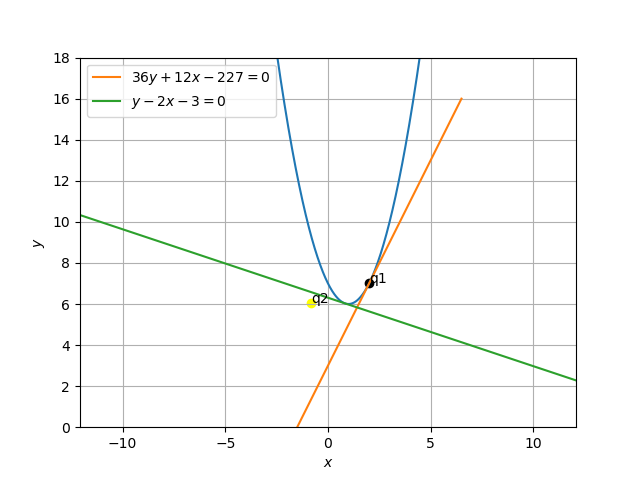
\includegraphics[scale=0.5]{conic.png}
\caption{Parabola}
\label{fig:Parabola}
\end{figure}
\end{flushleft}
\end{flushleft}
\end{document}
